\documentclass[12pt,a4paper]{article}

% --- PACKAGES ---
\usepackage[utf8]{inputenc}
\usepackage[T1]{fontenc}    % Add font encoding
\usepackage{amsmath}
\usepackage{amsfonts}       % Add math fonts package
\usepackage{amssymb}        % Add math symbols package
\usepackage{graphicx} % Required for including images
\usepackage[a4paper, margin=1in]{geometry} % For page margins
\usepackage{times} % Uses Times New Roman like font, similar to many academic papers
\usepackage{setspace}       % For line spacing
\usepackage{hyperref} % For clickable links in ToC and references
\hypersetup{
    colorlinks=true,
    linkcolor=RoyalBlue,  % previously "blue"
    filecolor=magenta,      
    urlcolor=cyan,
    pdftitle={DENDRAL Expert System Report},
    pdfpagemode=FullScreen,
}

\usepackage{fancyhdr} % For custom headers and footers
\usepackage{lipsum} % For placeholder text, remove in final version
\usepackage{caption}        % For customizing captions
\usepackage{subcaption}     % For subfigures
\usepackage{float}          % For better figure placement with [H]
\usepackage{tikz}
\usetikzlibrary{shapes.geometric, arrows, positioning, fit}

\usepackage{xcolor}
\usepackage{sectsty}
\usepackage{tocloft}

\definecolor{RoyalBlue}{RGB}{0, 0, 128}
\sectionfont{\color{RoyalBlue}}  % Section titles in document

% Table of Contents styling
\renewcommand{\cfttoctitlefont}{\color{black}\Huge\bfseries}    % Title "Contents" in black
\renewcommand{\cftsecfont}{\color{RoyalBlue}}                   % Section entries in ToC
\renewcommand{\cftsecpagefont}{\color{RoyalBlue}}               % Section page numbers
\renewcommand{\cftsubsecfont}{\color{RoyalBlue}}                % Subsection entries
\renewcommand{\cftsubsecpagefont}{\color{RoyalBlue}} 

% --- STYLING SIMILAR TO REFERENCE ---

% Page style for content pages
\pagestyle{fancy}
\fancyhf{} % Clear all header and footer fields
\fancyhead[C]{\textit{DENDRAL: AI in Chemical Structure Elucidation}} % Custom header
\fancyfoot[C]{\thepage}
\renewcommand{\headrulewidth}{0.4pt}
\renewcommand{\footrulewidth}{0pt} % No footer rule

% Title page command
\newcommand{\maketitlepage}{
    \begin{titlepage}
        \centering
        \vspace*{0.5cm}
        % 
\includegraphics[width=0.3\textwidth]{RUET_logo.png} % Replace RUET_logo.png with your university logo file
        {\Huge \textbf{RAJSHAHI UNIVERSITY OF ENGINEERING \& TECHNOLOGY}} % University Name
        \vspace*{0.5cm}
        {\Large Department of Computer Science and Engineering}
        
        \vspace*{2.5cm} % Vertical space
        
        {\huge\bfseries DENDRAL: Pioneering AI in Chemical Structure Elucidation\par}
        \vspace{0.5cm}
        {\Large \textit{A Comprehensive Analysis of an AI Expert System}\par}
        
        \vspace{2cm} % Vertical space
        
        \begin{flushleft}
        \large \textbf{Submitted by:}\\
        \large Md Naim Parvez \\ % <<< YOUR NAME HERE
        \large Roll No: 2003015 \\ % <<< YOUR ROLL NUMBER HERE
        \large Section: A \\ % <<< YOUR SECTION HERE
        \large Third Year (Even Semester) \\
        \end{flushleft}
        
        \vspace{1cm} % Vertical space
        
        \begin{flushleft}
        \large \textbf{Submitted to:}\\
        \large Md. Nasif Osman Khansur \\ % <<< LECTURER'S NAME HERE
        \large Lecturer \\ % <<< LECTURER'S DESIGNATION HERE
        \large Department of Computer Science and Engineering \\
        \large Rajshahi University of Engineering \& Technology (RUET) \\
        \end{flushleft}
        
        \vspace{1cm}
        {\large \textbf{Course Code:} CSE 3207} \\ % <<< COURSE CODE HERE (Example from friend's)
        {\large \textbf{Course Title:} Artificial Intelligence} % <<< COURSE TITLE HERE (Example from friend's)
        
        \vfill % Pushes content to bottom
        
        {\large June, 2025\par} % Submission Date
    \end{titlepage}
}

\begin{document}

% --- TITLE PAGE ---
\maketitlepage
\thispagestyle{empty} % No header/footer on the title page

% --- TABLE OF CONTENTS ---
\newpage
\pagenumbering{roman} % Roman numerals for ToC, Abstract etc.
\tableofcontents
\newpage
\pagenumbering{arabic} % Arabic numerals for main content
\setcounter{page}{1} % Start main content page numbering from 1

% --- I. REPORT TITLE (Already on Title Page) ---

% --- II. INTRODUCTION ---
\section{Introduction}
A major subfield of artificial intelligence (AI) expert systems are meant to replicate the capacity for decision-making of a human expert in a particular, limited field. These are computer programs that use knowledge and inference processes to address usually human-requiring problems. Expert systems in artificial intelligence serve primarily to capture rare hu-man knowledge and make it generally available, offer consistent and reliable decision-making, and help with difficult problem-solving chores. Usually they consist of an inference engine using the knowledge of the expert to derive conclusions from a knowledge base where his knowledge is kept.
\\\\This paper addresses ** DENDRAL**, one of the first and most effective expert systems that transformed the chemical structure elucidating process.
% --- III. BACKGROUND OF THE SELECTED EXPERT SYSTEM ---
\section{Background of DENDRAL}
DENDRAL (an acronym for "Dendritic Algorithm") was a groundbreaking project in artificial intelligence initiated in the mid-1960s at Stanford University. Important players in its evolution are Edward Feigenbaum, Bruce Buchanan, Joshua Lederberg (a Nobel laureate in genetics with a strong passion for using computational techniques to chemistry), and eminent chemist Carl Djerassi.
\\DENDRAL was driven mostly to help organic chemists find unknown organic compounds. It was intended especially to interpret mass spectrometry data.
A potent analytical method, mass spectrometry bombards a sample with electrons to cause molecules to fragment. The resultant fragment mass pattern—that of the mass spectrum—showcases a molecular signature. But determining the original molecular structure from this spectrum is a difficult combinatorial challenge that usually calls both great human knowledge and intuition. DENDRal sought to speed up and systemically automate this process. Thus, the domain was **organic chemistry** with an eye toward **molecular structure** from mass spectral data**
% --- IV. LITERATURE REVIEW ---
\section{Literature Review}
While DENDRAL itself was developed from the 1960s through the 1970s, its impact on AI and cheminformatics has been lasting, influencing subsequent research and system development. Early publications by its creators detailed its heuristic search algorithms and knowledge representation strategies (e.g., \cite{feigenbaum_lederberg1968}; \cite{buchanan1969}).
Lately, views on DENDRAL have focused on it as
showing that AI could address real-life scientific issues and make progress
Sources (Lindsay et al., 1980, 1993). The way it represents knowledge and searches for solutions
helped make other expert systems possible. Modern chemistry uses a wide variety
these include computational tools such as machine learning and quantum chemistry calculations.
the basic idea of using and organizing chemical knowledge, as first developed by DENDRAL is still considered valuable. Many studies in cheminformatics and drug discovery are now being performed in the present.
includes using hybrid methods that mix advanced machine learning techniques with established rules.
Founded on scientific principles from chemistry, as is true of DENDRAL’s quest for knowledge.
intensive problem-solving. Prioritizing the creation of many structurally feasible candidate molecules
In modern science, the practice of testing ideas by comparing them with data endures.
% --- V. ARCHITECTURE AND COMPONENTS ---
\section{Architecture and Components}
DENDRAL's architecture was innovative for its time and consisted of several key components, broadly fitting the expert system model:

\subsection{Knowledge Base}
Chemical experts had contributed a lot of knowledge to the DENDRAL system. This was not only
Not a pile of raw data, but organized rules and boundaries regarding organic chemistry. It
included:\begin{itemize}
    \item \textbf{Rules of mass spectrometry:} How different molecular structures and functional groups tend to fragment under electron bombardment. These rules helped predict how a candidate molecule might break apart, allowing comparison with the experimental spectrum
    \item \textbf{General chemical knowledge:} Rules about valency (how many bonds an atom can form), stability of chemical structures (e.g., avoiding highly strained rings unless evidence suggests them), and the properties of various functional groups.
    \item \textbf{Constraints from other spectroscopic data:} Even though the main science is mass spectrometry
DENDRAL had the ability to add data from additional approaches such as Nuclear Mag.
when NMR is available, to limit the variety of structures that are possible
    \item \textbf{CONGEN's constraints:} DENDRAL includes a system called CONGEN (CONstrained GENerator).
Created a graph-based approach to include every possibility for molecular isomers
Using an experimental formula and optionally including user-specified restrictions (such as requiring certain substructures)
\end{itemize}
This knowledge was encoded in a way that the system could use it to generate and prune candidate structures.

\subsection{Inference Engine}
DENDRAL's inference engine employed a "plan-generate-test" strategy:
\begin{enumerate}
    \item \textbf{Planning (DENDRAL-Planner):} This phase required analyzing the mass spectrum to determine what the possible molecular structures could be. It relied on heuristics to spot repeated forms in the spectrum that made it likely that specific substructures or functional groups were present. For instance, seeing a change in the mass can sometimes mean a methyl group (CH$_3$) or a water molecule (H$_2$O) was lost. Here, the searchable solutions were dramatically limited.
    \item \textbf{Generating (CONGEN/Generator):} The generator component (initially CONGEN), working with the limits set by the planner and any additional user constraints like the molecular formula, built every possible isomer. Molecules were represented by graphs, where the atoms made up the nodes and the bonds created the edges and special algorithms were applied to guarantee that every possible structure was included and no repetition occurred.
    \item \textbf{Testing (Tester/Predictor):} Each candidate structure produced was sent to the tester. Based on the knowledge, this component created a mass spectrum for the candidate molecule following the rules for fragmenting the molecule. Then, the results from the prediction were checked against the actual experimental spectrum. Those whose calculated spectra corresponded well with the real results were ranked above others.
\end{enumerate}
The reasoning was primarily heuristic search and rule-based deduction. It didn't use backward chaining in the same way as MYCIN; its approach was more constructive (building solutions) and then evaluative.

\subsection{User Interface}
The user interface for DENDRAL was relatively simple by today's standards, typical of systems from that era. Users (chemists) would typically interact with it via a teletype or terminal.
\begin{itemize}
    \item \textbf{Input:} The primary input was the empirical formula of the unknown compound and its mass spectrum data (a list of mass/intensity pairs). Users could also input additional constraints, such as known structural features or data from other spectroscopic methods (e.g., NMR).
    \item \textbf{Output:} The system would output a ranked list of candidate molecular structures that were consistent with the provided data and chemical knowledge.
    \item \textbf{Interaction:} While not as interactive with explanations as MYCIN's "why" questions, DENDRAL's process was somewhat transparent in that the constraints used by CONGEN were explicit, and the rules used by the predictor could be examined (though this might require more expert knowledge of the system itself).
\end{itemize}

\begin{figure}[h!]
    \centering
    % Replace the following line with your actual image file if available:
    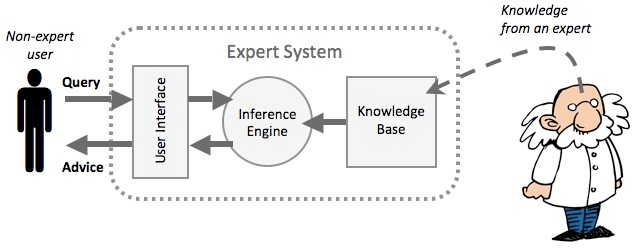
\includegraphics[width=0.7\textwidth]{expert-system.png}
    \caption{High-level Architecture of the DENDRAL Expert System.}
    \label{fig:dendral_architecture}
\end{figure}

% --- VI. WORKING MECHANISM ---
\section{Working Mechanism}
The working mechanism of DENDRAL followed the "plan-generate-test" paradigm:

\begin{enumerate}
    \item \textbf{Data Input:} The chemist provides the system with the unknown compound's mass spectrum data and its molecular formula. Optional inputs include data from other spectroscopic analyses (like NMR) or known constraints about the molecule (e.g., "it contains a benzene ring" or "it does not contain any oxygen atoms").
    
    \item \textbf{Planning Phase (DENDRAL-Planner):}
        \begin{itemize}
            \item The planner analyzes the input mass spectrum to identify characteristic fragmentation patterns or peaks.
            \item It applies heuristic rules derived from expert chemists' knowledge about how different molecular substructures (functional groups, types of bonds) behave in a mass spectrometer.
            \item This phase results in a set of constraints or inferences about the likely presence or absence of certain substructures in the unknown molecule. For example, a strong peak at m/z = M-15 might suggest the loss of a methyl group.
        \end{itemize}

    \item \textbf{Structure Generation Phase (CONGEN/Generator):}
        \begin{itemize}
            \item Using the molecular formula and the constraints derived from the planning phase (and any user-defined constraints), the CONGEN program systematically generates all possible chemical structures (isomers) that fit these criteria.
            \item It represents molecules as graphs and uses algorithms to ensure that all valid structures are generated without redundancy and that chemically impossible structures are avoided (e.g., atoms with too many bonds). This is a constrained graph generation problem.
        \end{itemize}
        
    \item \textbf{Structure Testing/Prediction Phase (Tester/Predictor):}
        \begin{itemize}
            \item For each candidate structure generated by CONGEN, the predictor module simulates its theoretical mass spectrum.
            \item This simulation is based on a large set of rules in the knowledge base that describe how different types of bonds and substructures within a given candidate molecule are likely to break under electron bombardment in a mass spectrometer.
            \item The predicted spectrum for each candidate is then compared against the original experimental mass spectrum provided by the user.
        \end{itemize}
        
    \item \textbf{Output and Ranking:}
        \begin{itemize}
            \item Candidate structures whose predicted mass spectra closely match the experimental spectrum are considered good candidates for the unknown compound.
            \item The system presents a ranked list of these plausible structures to the chemist for further review and confirmation, typically with the best matches ranked highest.
        \end{itemize}
\end{enumerate}

The reasoning techniques used include:
\begin{itemize}
    \item \textbf{Heuristic Search:} The planner uses heuristics to narrow down the search space of possible structures.
    \item \textbf{Generate and Test:} This is the overarching paradigm. CONGEN generates potential solutions, and the Tester evaluates them.
    \item \textbf{Rule-Based Reasoning:} The Planner and Tester components rely heavily on IF-THEN rules that encapsulate chemical knowledge.
    \item \textbf{Constraint Satisfaction:} CONGEN generates structures that satisfy a set of constraints (elemental composition, presence/absence of substructures).
\end{itemize}

\begin{figure}
    \centering
    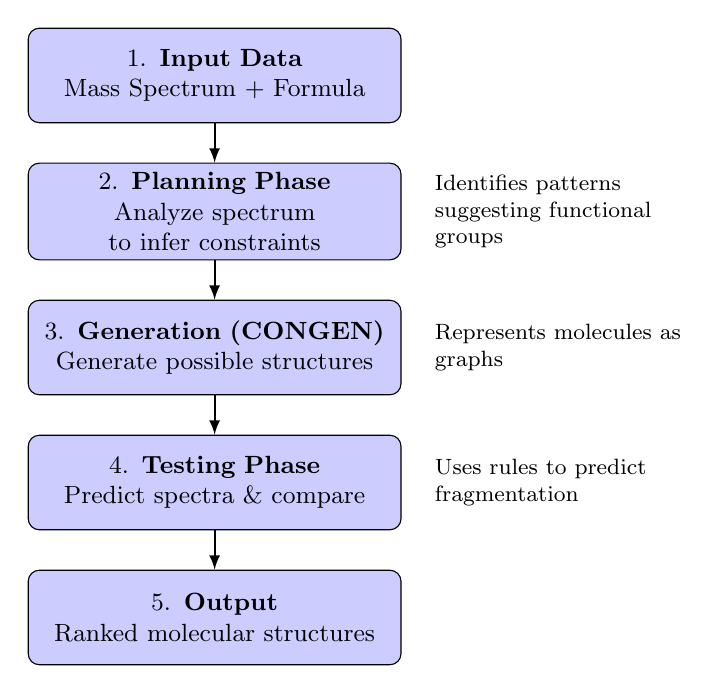
\begin{tikzpicture}[
        block/.style={rectangle, draw, fill=blue!20, text width=4.5cm, text centered, rounded corners, minimum height=1.2cm, font=\small},
        line/.style={draw, -latex, thick},
        note/.style={text width=3.2cm, align=left, font=\footnotesize}
    ]
    
    % Nodes - reduced spacing and text width
    \node[block] (input) {1. \textbf{Input Data}\\Mass Spectrum + Formula};
    \node[block, below=0.5cm of input] (plan) {2. \textbf{Planning Phase}\\Analyze spectrum to infer constraints};
    \node[block, below=0.5cm of plan] (generate) {3. \textbf{Generation (CONGEN)}\\Generate possible structures};
    \node[block, below=0.5cm of generate] (test) {4. \textbf{Testing Phase}\\Predict spectra \& compare};
    \node[block, below=0.5cm of test] (output) {5. \textbf{Output}\\Ranked molecular structures};
    
    % Connections
    \path [line] (input) -- (plan);
    \path [line] (plan) -- (generate);
    \path [line] (generate) -- (test);
    \path [line] (test) -- (output);
    
    % Side annotations - reduced text and font size
    \node[note, right=0.3cm of plan] {Identifies patterns suggesting functional groups};
    \node[note, right=0.3cm of generate] {Represents molecules as graphs};
    \node[note, right=0.3cm of test] {Uses rules to predict fragmentation};
    
    \end{tikzpicture}
    \caption{Working Mechanism of DENDRAL: Plan-Generate-Test Strategy}
    \label{fig:dendral_workflow}
\end{figure}

% \newpage
% --- VII. STRENGTHS AND LIMITATIONS ---
\section{Strengths and Limitations}

\subsection{Strengths}
\begin{itemize}
    \item \textbf{Pioneering Success:} DENDRAL was one of the first expert systems to achieve expert-level performance in a complex scientific domain. It demonstrated that AI could tackle real-world problems and codify specialized human knowledge.
    \item \textbf{Systematic Structure Elucidation:} It provided a systematic and exhaustive approach to identifying molecular structures, often outperforming human chemists in terms of speed and the number of possibilities considered, especially for certain classes of molecules.
    \item \textbf{Knowledge Codification:} The project was highly successful in articulating and codifying the heuristic knowledge of expert chemists into a machine-usable format. This was a significant contribution to knowledge engineering.
    \item \textbf{Influence on AI:} DENDRAL's "plan-generate-test" paradigm and its techniques for knowledge representation and heuristic search influenced many subsequent expert systems and AI research projects.
    \item \textbf{Educational Value:} The rules and models developed for DENDRAL also contributed to a better understanding of mass spectrometry and chemical structure.
\end{itemize}

\subsection{Limitations}
\begin{itemize}
    \item \textbf{Narrow Domain:} Like most early expert systems, DENDRAL's expertise was confined to a very specific task (elucidating structures of acyclic organic compounds, primarily from mass spectrometry). It was not a general chemistry problem solver.
    \item \textbf{Knowledge Acquisition Bottleneck:} While successful, acquiring and formalizing the chemical knowledge and fragmentation rules was a labor-intensive process, requiring close collaboration between chemists and AI researchers over many years.
    \item \textbf{Computational Intensity:} For its time, generating and testing a large number of candidate structures could be computationally expensive, though this became less of an issue with advancing hardware.
    \item \textbf{Reliance on Mass Spectrometry:} Its primary strength was with mass spectrometry data. While it could incorporate other data, its core reasoning was built around MS. If MS data was poor or ambiguous, its performance suffered.
    \item \textbf{Novel Structures/Rules:} It could struggle with entirely novel chemical structures or fragmentation pathways that were not covered by its existing rule set. Updating the knowledge base was a non-trivial task.
    \item \textbf{User Interface:} The teletype-based interface was not very user-friendly by modern standards, limiting its accessibility to some extent.
\end{itemize}

% --- VIII. APPLICATIONS AND IMPACT ---
\section{Applications and Impact}
While DENDRAL itself was primarily a research project at Stanford University and wasn't commercialized into a widely distributed software product in the same way some later systems were, its applications and impact were profound:
\begin{itemize}
    \item \textbf{Real-World Problem Solving:} DENDRAL was successfully used to elucidate the structures of numerous unknown organic compounds, particularly for classes of molecules like aliphatic amines, ethers, and ketones. It helped chemists in their research work.
    \item \textbf{Validation of AI:} It served as a powerful demonstration of the potential of AI and expert systems, showing that computers could perform tasks requiring deep expert knowledge and reasoning. This boosted confidence and funding in the AI field.
    \item \textbf{Foundation for Cheminformatics:} DENDRAL laid some of the foundational groundwork for the field of cheminformatics (or chemoinformatics), which applies computational and informational techniques to a range of problems in chemistry.
    \item \textbf{Spin-off Projects:} The success of DENDRAL led to other related expert systems and AI projects in chemistry and other scientific disciplines, such as META-DENDRAL, which focused on automatically learning new rules for mass spectrometry.
    \item \textbf{Influence on Heuristic Programming:} The "Heuristic DENDRAL" project significantly advanced the understanding of how to build programs that could solve complex problems using heuristic search and domain-specific knowledge.
    \item \textbf{Educational Impact:} The process of building DENDRAL helped to formalize and clarify many aspects of mass spectral interpretation, which was valuable for teaching and understanding the field.
\end{itemize}

\textbf{Modern Successors and Influence:}
While direct "successors" that are simply updated versions of DENDRAL are not common, its legacy is seen in:
\begin{itemize}
    \item \textbf{Computer-Assisted Structure Elucidation (CASE) Systems:} Modern CASE systems use sophisticated algorithms, often combining multiple spectroscopic data types (MS, NMR, IR, UV-Vis), and may incorporate machine learning techniques alongside rule-based approaches. Examples include ACD/Structure Elucidator.
    \item \textbf{Fragment Libraries and Spectral Databases:} The idea of matching spectral features to structural fragments is fundamental to modern spectral database searching (e.g., NIST, Wiley).
    \item \textbf{Quantitative Structure-Activity Relationship (QSAR) models and Drug Discovery Tools:} These tools often rely on representing molecular structures and predicting properties, a conceptual descendant of DENDRAL's approach.
\end{itemize}
DENDRAL's core contribution was demonstrating the power of encoding specialized knowledge to solve complex scientific problems, a principle that continues to be relevant in modern AI applications across various domains.

% --- IX. CONCLUSION ---
\section{Conclusion}
In the history of artificial intelligence, DENDRAL is considered a significant breakthrough and shows the capabilities of expert systems. This first success of automating a tough scientific function, explaining chemical structures from mass spectrometry data, was a key boost for the AI field. We realized that computers could both do calculations and also do complex reasoning, tasks we thought were special abilities of human experts.

The key lessons learned from the DENDRAL project are multifaceted:
\begin{itemize}
    \item \textbf{Power of Domain-Specific Knowledge:} DENDRAL highlighted that deep, specialized knowledge is crucial for expert-level performance. Its strength came from its extensive knowledge base of chemical rules and heuristics.
    \item \textbf{The "Plan-Generate-Test" Paradigm:} This proved to be an effective problem-solving strategy for complex domains where the search space is vast.
    \item \textbf{Knowledge Engineering Challenges:} The project underscored the "knowledge acquisition bottleneck" – the difficulty and labor-intensiveness of eliciting, formalizing, and encoding expert knowledge.
    \item \textbf{Feasibility of AI in Science:} DENDRAL opened the door for numerous other AI applications in scientific discovery and analysis.
\end{itemize}
DENDRAL may no longer exist as a system, but the things learned from it continue to guide research and application in AI, cheminformatics and scientific expert systems. This project serves as a key example showing how AI supports human reasoning and tries to address big practical concerns.


\newpage
% --- X. REFERENCES ---
\section*{References}
\renewcommand{\refname}{\vspace{-1em}} % Removes the default "References" title if you use \section*
\begin{thebibliography}{99}
    % --- Remember to find appropriate references for DENDRAL ---
    % Example format:
    \bibitem{buchanan1969}
    Buchanan, B. G., Sutherland, G. L., \& Feigenbaum, E. A. (1969). Heuristic DENDRAL: a program for generating explanatory hypotheses in organic chemistry. In Meltzer, B., Michie, D., \& Swann, M. (Eds.), \textit{Machine Intelligence 4}. Edinburgh University Press.
    
    \bibitem{lindsay1980}
    Lindsay, R. K., Buchanan, B. G., Feigenbaum, E. A., \& Lederberg, J. (1980). \textit{Applications of artificial intelligence for organic chemistry: The DENDRAL project}. McGraw-Hill.
    
    \bibitem{lindsay1993}
    Lindsay, R. K., Buchanan, B. G., Feigenbaum, E. A., \& Lederberg, J. (1993). DENDRAL: a case study of the first expert system for scientific hypothesis formation. \textit{Artificial Intelligence}, 61(2), 209-261.
    
    \bibitem{feigenbaum_lederberg1968}
    Lederberg, J., \& Feigenbaum, E. A. (1968). Mechanization of inductive inference in organic chemistry. In Klein, B. \& G. W. (Eds.), \textit{Formal Representation of Human Judgment}. Wiley. (Often cited as a foundational paper, though exact proceedings titles can vary in records).
    
    \bibitem{russell_norvig_ai} % General AI textbook reference
    Russell, S. J., \& Norvig, P. (2020). \textit{Artificial Intelligence: A Modern Approach} (4th ed.). Pearson.
    
    % --- Add more relevant references here ---
    % For example, papers on CONGEN, Meta-DENDRAL, or reviews of DENDRAL.

\end{thebibliography}

\end{document}